\documentclass{article}
\usepackage[utf8]{inputenc}
\usepackage{graphicx}
\usepackage{float} 
\usepackage{array}
\textheight 24cm
\textwidth 16cm
\oddsidemargin 0cm
\evensidemargin 0cm
\topmargin 0cm
\hoffset -0mm
\voffset -20mm
\usepackage[]{listings}
\usepackage{amsmath}
\title{Geometric Modeling}
\author{Manuel Camargo & Mohamed Traoré &  Nicolas Gindrier}
\date{}
\begin{document}

\maketitle
\section*{Summary and presentation}
\begin{figure}[H]
   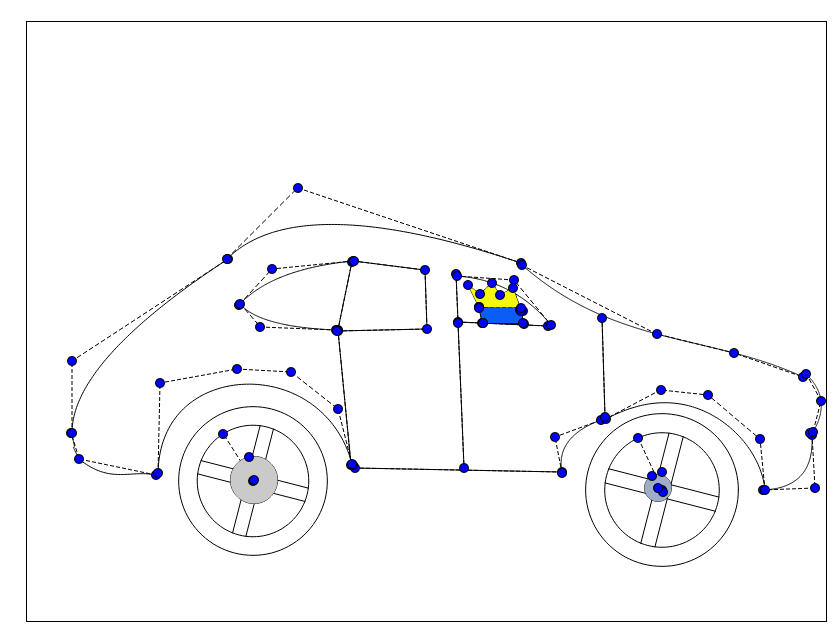
\includegraphics[scale = 0.5]{Pictures/narutovoiture.png}
\end{figure}
\section*{Organization}
We used Github.
\section*{Curves}
\subsection*{Curves 1-D}
\subsection*{Curves 2-D}
\subsubsection*{Bezier-Aitken}
\begin{figure}[H]
   \includegraphics[scale = 0.5]{Pictures/bezier-aitken.png}
\end{figure}
\subsubsection*{Hermite-Hermite closed}
\begin{figure}[H]
   \includegraphics[scale = 0.5]{Pictures/hermite.png}
\end{figure}
\subsubsection*{Wheel-Gear}
\begin{figure}[H]
   \includegraphics[scale = 0.5]{Pictures/gear-wheel.png}
\end{figure}

\subsection*{others} %for example DelCurve
\section*{Prospects}
We had a lot of ideas but some of them have not been made. It was because of timme, or because we fear to modify some files. We do not master the architecture of the whole project. 
\end{document}
